\documentclass[tikz, margin=3mm]{standalone}

\begin{document}
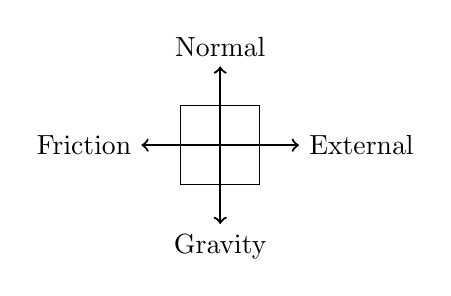
\begin{tikzpicture}
    % Draw the square (object)
    \draw (0,0) rectangle (1,1);
    
    % Draw the forces (arrows)
    \draw[->, thick] (0.5,0.5) -- (0.5,-0.5) node[below] {Gravity};
    \draw[->, thick] (0.5,0.5) -- (0.5,1.5) node[above] {Normal};
    \draw[->, thick] (0.5,0.5) -- (-0.5,0.5) node[left] {Friction};
    \draw[->, thick] (0.5,0.5) -- (1.5,0.5) node[right] {External};
\end{tikzpicture}
\end{document}